Within this chapter the general design of the system implementing the new process is described. First of al the general design is discussed, followed by a explanation about the used languages and frameworks. Finally, the rule set request is explained. 

\section{General Design}
Due to the fact that the system should be a web application, a modified \gls{mvc} is used to split up business logic and the user interface presentation. The system has the following components:

\begin{table}[h!]
	\begin{tabular}{|p{4cm}|p{11cm}|} \hline
		Component & Functionality \\ \hline
		View & Presents the result of the  business logic and triggers the user interaction.\\ \hline
		Controller & Handles the communication between view and service in such a way, that the other components do not need to know from each other. The controller process all transmitted actions from the view and request the service for the corresponding tasks. The returned information are prepared for the view and presented through the view to the user. \\ \hline
		Service & This component holds the business logic of the system and coordinates the interactions with the \frqq information\flqq components. \\ \hline
		Model & \\ \hline
		\Gls{erp} Connector & It is responsible for the communication with the \gls{erp}. As information it has to provide information about documents, customer and the employee uploaded the document. \\ \hline
		Signing Tool Connector & \\ \hline
		User Reader & \\ \hline
		Rules Reader & \\ \hline
	\end{tabular}
	\centering
	\caption{Listing of Systems Components}
	\label{tab:listingSystemComponents}
\end{table}
\begin{figure}[h!]
	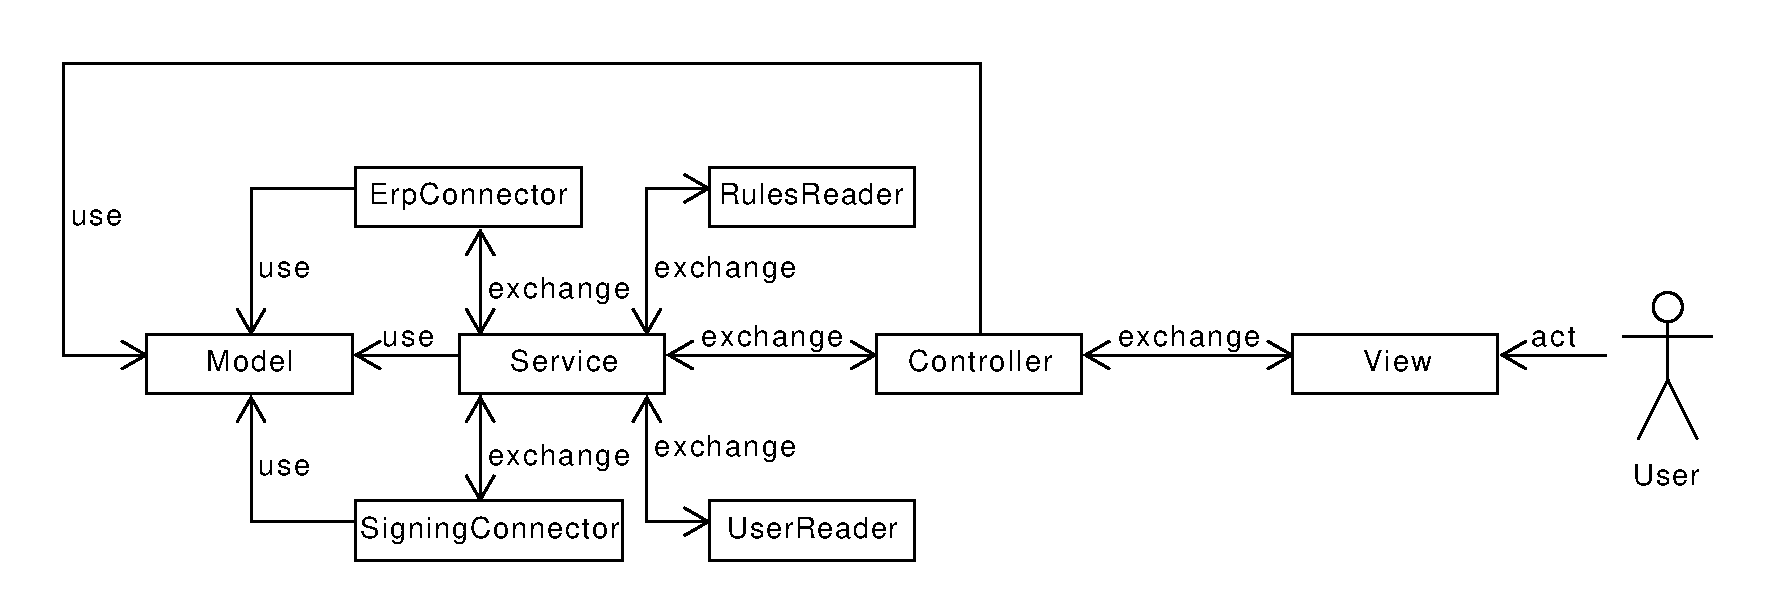
\includegraphics[width=\linewidth]{./design/images/generalCommunication.pdf}
	\caption{General system design}
	\label{fig:generalDesign}
\end{figure}

\subsection*{Enterprise Resource Planning System Connection}
- as variable as possible for ERp systems -> interface specify methods for system

\subsection*{Rule Reader Connection}
- as variable as possible for rule set storage -> interface because every company could have own preferences

\subsection*{Signing Tool Connection}
- as variable as possible for signing tool -> could be changed based on new requirements or company depending: interface

\subsection*{User Reader Connection}
- user management via interface, cause every company could already have existing and to reduce maintenance of data in several dbs 

\section{Used Programming Language and Frameworks}
- why used discussion
- first idea js, but less expiriences not all tools have all functionalities inside Rest api
- Java 8: in company widely used, a lot of experience, time constrains, most SDks available or REST API
- Spring Boot: easy set up, has already a lot of functionalities like security log in, embedded dbs / server, get new experiences, server configurations
- Maven: regulates the dependencies of project, can be build on every machine where maven and java is installed

\begin{table}[h!]
	\begin{tabular}{|l|c|c|} \hline
		Framework/ Tool & Functionality & Usage \\ \hline
		Maven & & \\ \hline
		Spring Boot & & \\ \hline
		Lombock & & \\ \hline
		Mockito & & \\ \hline
		h2 & & \\ \hline
		DocuSign eSign & & \\ \hline
	\end{tabular}
	\centering
	\caption{List used Frameworks}
	\label{tab:frameworks}
\end{table}

\section{Rule Set Request}
Inside the rule set the signing guideline is stored for the system. In general it can be said that there exist four general data sets:
\begin{itemize}
	\item Company positions: \newline
	Inside this data set all the positions of a company are listed, which can be allocated in the company. Each of them has different rights and liabilities.
	\item Document types: \newline
	At a company several different document types exists and they need to be handled differently regarding the signatures. 
	\item Value ranges: \newline
	In a signing guideline several different value ranges are listed. They are inserted in this data set. Each of them has a minimum value and a maximum value.
	\item Signing groups: \newline
	Inside a company several signing groups exists, which consist of different company positions. Each group has combined rights.
\end{itemize}

The rule set is a combination of the previous explained data sets. It defines for each document type and the corresponding value ranges which signing group is allowed to sign the combination. \newline
In the situation a user selects a document for signing, the system needs to analyze based on the document type, the value of the document and the position of the user, if the user is allowed to sign at all and if yes are there other company positions that need to sign along. 

The mathematical presentation of this request is presented in the appendix \ref{mathCode} and the visualization in the appendix \ref{visuRuleset}. ---ToDo: viulization----

\subsection*{Example}
For a better understanding the previous explained theoretical an example is given based on the signing guideline from \gls{cc} presented in table \ref{tab:newSigningGuideline}: \newline
The general data sets:
\begin{itemize}
	\item Company positions: employee; salesman; manager; procurator; chairman
	\item Document types: quotation; \gls{nda}; contract
	\item Value ranges: 0 - 50 000; 50 000,01 - 400 000; 400 000,01 - $\infty$; 0 - $\infty$
	\item Signing groups (extracts): employee only; manager only; salesman with manager; manager with chairman; ....
\end{itemize}

For the rule set example also an extract is selected. In the following the entries are presented:
\begin{enumerate}
	\item Contract; (0 - 50 000); salesman alone
	\item Contract; (0 - 50 000); manager alone
	\item Contract; (0 - 50 000); chairman alone
	\item Contract; (50 000,01 - 400 000); salesman with manager
	\item Contract; (50 000,01 - 400 000); salesman with chairman
	\item Contract; (50 000,01 - 400 000); manager alone
	\item Contract; (50 000,01 - 400 000); chairman alone
	\item Contract; (400 000,01 - $\infty$); salesman with chairman
	\item Contract; (400 000,01 - $\infty$); manager with chairman
	\item Contract; (400 000,01 - $\infty$); chairman alone
\end{enumerate}